\documentclass[a4paper]{article}

%% Language and font encodings
\usepackage[english]{babel}
\usepackage[utf8x]{inputenc}
\usepackage{natbib}
\usepackage{booktabs}
\usepackage{tabu}
\usepackage[T1]{fontenc}

%% Sets page size and margins
\usepackage[a4paper,top=3cm,bottom=2cm,left=3cm,right=3cm,marginparwidth=1.75cm]{geometry}

%% Useful packages
\usepackage{amsmath}
\usepackage{graphicx}
%\usepackage{apacite}
\usepackage[colorinlistoftodos]{todonotes}
\usepackage[colorlinks=true, allcolors=blue]{hyperref}

\title{Network-based Protein Function Prediction via Deep Graph Convolutional Neural Networks}
\author{MSc. Vicente Enrique Machaca Arceda}
\date{\today}

\begin{document}
\maketitle

\section{Introduction}

Protein assemblies are modules of Protein-Protein Interactions (PPI), they coordinate the execution of all biochemical, signaling, and functional processes in cells \citep{alberts1998cell}. Moreover, protein assemblies are in order of hundreds, for example, the single-cell \textit{Saccharomyces cerevisiae} has more than 400 assemblies \citep{srihari2017computational}. Also, it is known that proteins interact physically with other proteins and biomolecules; for instance, over 80\% of proteins not function alone, they work as macromolecular assemblies \citep{berggaard2007methods}. Furthermore, with new low-cost protein sequencing technologies, there is a massive growth of sequences available, for example, UniProt has 100 million sequences and only 0.5 million are manually annotated (the rest are unlikely to be experimentally characterized) \citep{gligorijevic2020structure}. Nowadays, the knowledge of functional roles of proteins is one of the most important problems in bioinformatic.\\

In this research proposal, we present a deep graph convolutional network to predict network-based protein functions. In Section \ref{stateart}, we present the most relevant works based on protein function prediction. Moreover, in Section \ref{proposal}, we present our proposal based on graph convolutional networks. 

\section{State of art}\label{stateart}

Network-based protein function prediction, used networks information. For instance, network-based protein structural, represent nodes are amino acids and edges link amino acids that are spatially close. For example, \cite{newaz2018network} and \cite{ghalehnovi2019novel}, used graphlets as features along with deep learning. \\

Another approach takes into account PPI networks; they consider proteins as nodes and edges represent the interaction between proteins. For example, \cite{freschi2007protein} annotated functions of protein interactions with a random walk algorithm. Also, \cite{vascon2020protein}, used a graph-transduction game. Moreover, \cite{vazquez2003global} used PPI networks to assigned the protein's function, according to the network physical interaction; they used their method to analyze the yeast \textit{Saccharomyces cerevisiae} PPI. Finally, there are some platforms, like NetGO, this tool used massive protein-protein network information to automated function prediction \citep{you2019netgo}. There is also, FunCoup, a web framework to infer genome-wide functional coupling \citep{ogris2018funcoup}.\\

Furthermore, several studies have been proposed in the field of PPI networks.  \cite{kovacs2019network} studied protein interactions, they offered structural and evolutionary evidence that proteins interact despite their dissimilarity. Moreover, \cite{jia2019ippi}, used Chaos Game Representations (CGR) to predict protein-protein interactions. Furthermore, the use of deep learning has been applied extensively to predict protein interactions \cite{wang2019predicting, zhang2019protein, zeng2020protein}.\\


\section{Proposal}\label{proposal}

In this research, a Graph Convolutional Neural Network (GCN)  is proposed for protein function prediction based on protein-protein interactions. I will apply the method proposed by \cite{Susha2019}, where a PPI network is represented as a weighted attributed graph, where each protein is represented as a node and protein-protein interactions are edges. Then, we will apply a series of convolutional layers followed by pooling layers. Finally, we will classify the network/graph with its corresponding function. We will use the databases proposed in \cite{you2019netgo}. \\

The convolution operation is the main challenge in this research. In this case, we need to find a new representation for each vertex by aggregating the attributes of its neighbors. \cite{Susha2019} update each vertex with information of the vertices in k-order proximity. For example in Figure \ref{fig:conv} (right), we represent the vertices in 1-order proximity of red vertex. 

\begin{figure}[hbt!]
	\centering
	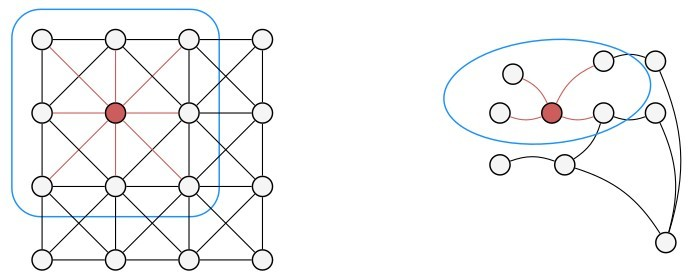
\includegraphics[width=0.6\textwidth]{img/conv.jpg}
	\caption{Analogous of convolution on images and graphs. Left: CNN operator for images. Right: CNN operator for graphs. Source: \cite{Susha2019}}
	\label{fig:conv}
\end{figure}

\subsection{Why am I interested  for the project?}
The knowledge of protein function and protein-protein interactions are the key point to understand the nature of biology. Classical methods are too expensive, nevertheless, computer science could help. I'm a computer science researcher passionate in the understanding of protein/gene functions and the future applications of this field.

\subsection{How will I complete the project?}

I have scheduled my activities. Also, I have defined milestones in order to accomplish the project (Table \ref{tab:act}). Now, I'm in the literature review and the implementation of the first method that is based on graph convolutional networks. Moreover, I planned to use autoencoders as the second method.

\begin{table}[hbt!]
	\caption{Activities for the research proposal.}
	\label{tab:act}
	\begin{tabular}{lcccc}
		\hline
		Activities                      & trimester 1 & trimester 2 & trimester 3 & trimester 4 \\ \hline
		Literature review             & x          & x          &            &            \\
		Method 1 implementation       & x          & x          &            &            \\
		Evaluation of results         &            & x          &            &            \\
		Paper redaction and submition &            & x          &            &            \\
		Method 2 implementation       &            & x          & x          &            \\
		Evaluation of results         &            &            &            & x          \\
		Paper redaction and submition &            &            &            & x         \\ \hline
	\end{tabular}
\end{table}

\subsection{What makes me suitable to complete the project?}
I have computer science aptitudes to accomplish the project. Moreover, I have experience in research projects. I consider myself, very passionate about the field of PPI networks and its applications, even if I were not selected, I am going to continue the research because is the field I choose to research.


\bibliographystyle{apalike}
\bibliography{bibliography}

\end{document}